\documentclass{article}
\usepackage[utf8]{inputenc}
\usepackage[spanish]{babel}
\usepackage{amsmath}
\usepackage{amssymb}
\usepackage{amsfonts}
\usepackage{hyperref}
\usepackage{textcomp}
\usepackage{graphicx}
\usepackage{pgfplots}
\usepackage{geometry}
\hypersetup{
    colorlinks=true,
    linkcolor=black,
    citecolor=green,
    filecolor=magenta,      
    urlcolor=cyan,
}
\geometry{
  top=3cm,            % Margen superior
  bottom=3cm,         % Margen inferior
  left=3cm,           % Margen izquierdo
  right=3cm           % Margen derecho
}

\title{Estadística 1}
\author{Jorge Miguel Alvarado Reyes}
\date{16 Agosto 2023}

\setlength{\parindent}{0pt}
\begin{document}

\begin{titlepage}
    \begin{center}
        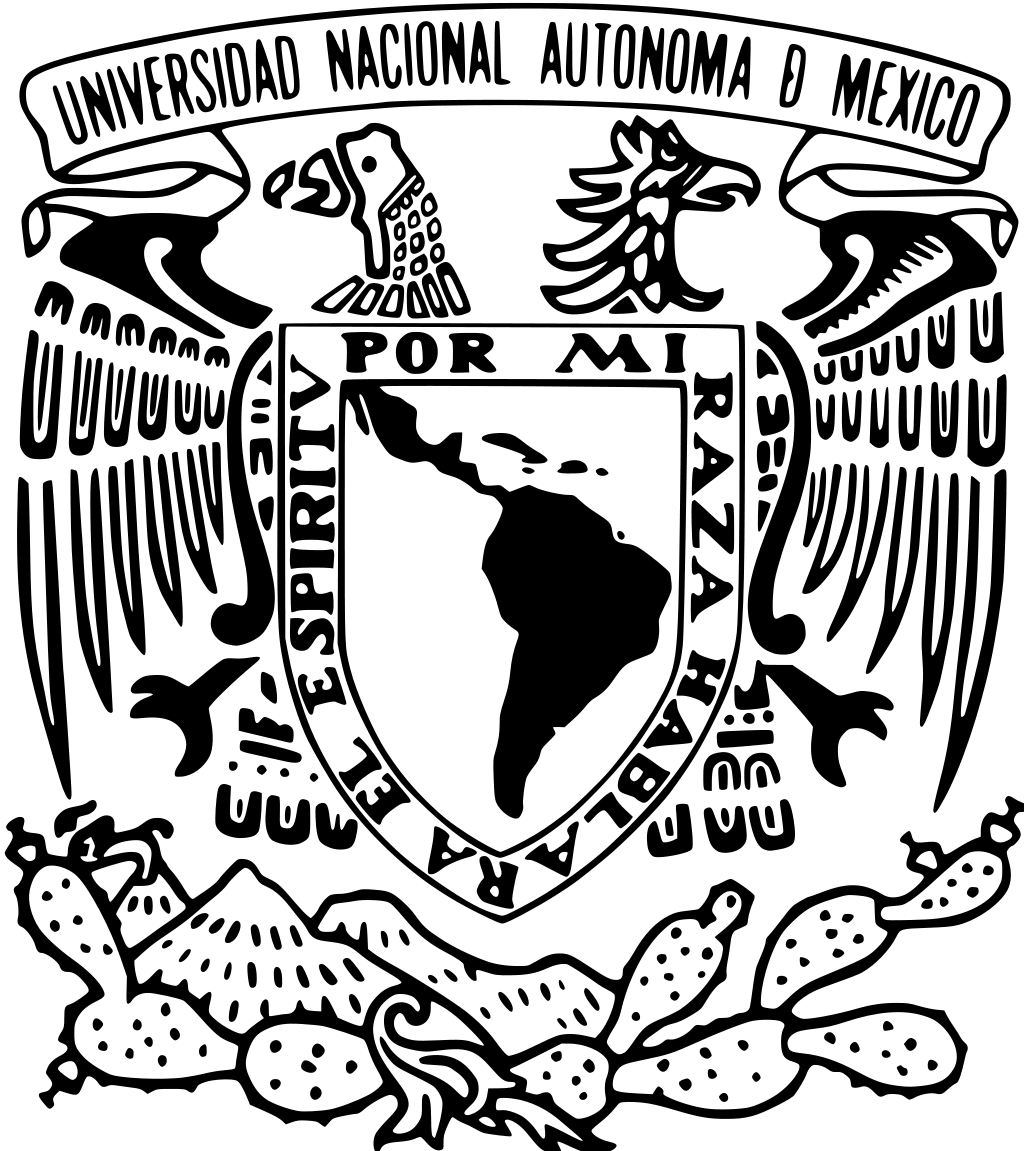
\includegraphics[width=0.2\textwidth]{../../unam.png}
        \vspace*{.5cm}

        \LARGE
        \textbf{Universidad Nacional Autónoma de México}

        \vspace{0.5cm}
        \LARGE
        Facultad de Estudios Superiores Acatlán

        \vspace{2cm}

        \textbf{Apuntes} \\
        Ecuaciones Diferenciales

        \vfill

        \vspace{1cm}

        \textbf{\large Autor:} \\
        Jorge Miguel Alvarado Reyes \\
        421010301\\
        \vspace{.5cm}
        \normalsize \today

    \end{center}
\end{titlepage}
\newpage

\tableofcontents


\section{Teoremas de la tranformada de laplace}

\[
    \mathcal{L}\{c\} = \frac{c}{s}
\]

\[
    \mathcal{L}\{t^n\} = \frac{n!}{s^{n+1}}
\]

\[
    \mathcal{L}\{sen(\alpha t)\} = \frac{\alpha}{s^2 + \alpha^2}
\]

\[
    \mathcal{L}\{cos(\alpha t)\} = \frac{s}{s^2 + \alpha^2}
\]

\[
    \mathcal{L}\{e^{\alpha t}\} = \frac{1}{s - \alpha}
\]

\[
    \mathcal{L}\{senh(\alpha t)\} = \frac{\alpha}{s^2 - \alpha^2}
\]

\[
    \mathcal{L}\{cosh(\alpha t)\} = \frac{s}{s^2 - a^2}
\]


\section{Tarea 4}

\begin{enumerate}
    \item $y' + 4y = e^{-4t}, \hspace{.5cm} y(0) = 2 \hspace{.5cm} y'(0)=0$
    \item $y' - y = 1 - te^{t}, \hspace{.5cm} y(0) = 0$
    \item $y'' + 2y' + y = 0, \hspace{.5cm} y(0) = y'(0) = 1$
    \item $y'' - 4y' + 4y = t^{3}e^{2t}, \hspace{.5cm} y(0) = y'(0) = 0 $
    \item $y'' - 6y' + 9y = t, \hspace{.5cm} y(0) = 0, y'(0) = 1$
    \item $y'' - 4y' + 4y = t^3, \hspace{.5cm} y(0) = 1, y'(0) = 0 $
    \item $y'' - 6y' + 13y = 0, \hspace{.5cm} y(0) = 0, y'(0) = -3$
    \item $2y'' + 20y' + 51y = 0, \hspace{.5cm} y(0) = 2, y'(0) = 0$
    \item $y'' - y' = e^{t}cos(t), \hspace{.5cm} y(0) = 0, y'(0) = 0 $
    \item $y'' - 2y' + 5y = 1 + t, \hspace{.5cm} y(0) = 0, y'(0) = 4$
\end{enumerate}

\newpage

\subsection{Solución}

\subsubsection{Problema 1}
\[y' + 4y = e^{-4t}, \hspace{.5cm} y(0) = 2\]

Aplicar la Transformada de Laplace en la ecuación es:
\begin{equation*}
    \mathcal{L}\{y'\} + 4\mathcal{L}\{y\} = \mathcal{L}\{e^{-4t}\}.
\end{equation*}

Resolviendo $\mathcal{L}\{e^{-4t}\}$:

\begin{align*}
    \mathcal{L}\{e^{-4t}\} & = \int_0^\infty e^{-st}e^{-4t}\,dt                  \\
                           & = \int_0^\infty e^{-(s+4)t}\,dt                     \\
                           & = \left[ -\frac{1}{s+4}e^{-(s+4)t} \right]_0^\infty \\
                           & = \frac{1}{s + 4}
\end{align*}

Resolviendo $\mathcal{L}\{y'\}$ y $\mathcal{L}\{y\}$
\begin{align*}
    \mathcal{L}\{y'\} & = sY(s) - y(0), \\
    \mathcal{L}\{y\}  & = Y(s),
\end{align*}

Sustituyendo con la condicion inicial \(y(0) = 2\) en la ecuación:
\begin{equation*}
    sY(s) - 2 + 4Y(s) = \frac{1}{s + 4}
\end{equation*}

Esto simplifica a:
\begin{equation*}
    Y(s)(s + 4) = 2 + \frac{1}{s + 4}
\end{equation*}

Despejamos \(Y(s)\):
\begin{equation*}
    Y(s) = \frac{2}{s + 4} + \frac{1}{(s + 4)^2}
\end{equation*}

\[
    Y(s) = \frac{2s+9}{(s + 4)^2}
\]

\[\frac{2s+9}{(s + 4)^2} = \frac{A}{s+4} + \frac{B}{(s+4)^2}\]

\[2s+9 = A(s+4) + B\]

\[2s+9 = As+4A + B\]

\[2s+9 = A(s+4) + B\]

Para $s=-4$

\[2(-4)+9 = A(-4+4) + B\]

\[-8 + 9 = A(0) + B\]

\[1 = B\]

Como sabemos que $B=1$

\[2s+9 = A(s+4) + 1\]

Para $s=1$

\[2(1)+9 = A(1+4) + 1\]

\[11 = A5 + 1\]

\[2 = A\]

Por lo tanto los valores de $A$ y $B$ son

\[A=2 \hspace{.5cm} B=1\]

\[\frac{2s+9}{(s + 4)^2} = \frac{2}{s+4} + \frac{1}{(s+4)^2}\]

Ahora aplicamos la tranfsormada inversa de laplace
\begin{align*}
    \mathcal{L}^{-1}\{\frac{2}{s+4}\} + \mathcal{L}^{-1}\{\frac{1}{(s+4)^2}\} = 2\mathcal{L}^{-1}\{\frac{1}{s+4}\} + \mathcal{L}^{-1}\{\frac{1}{(s+4)^2}\}
\end{align*}

Sabemos:

\[ \mathcal{L}^{-1}[\frac{1}{s-a}] = e^{at} \hspace{1cm} \mathcal{L}^{-1}[\frac{1}{(s-a)^n}] = \frac{t^{n-1}e^{at}}{(n-1)!}\]

Por lo tanto:

\begin{align*}
    \mathcal{L}^{-1}\left\{\frac{2}{s+4}\right\} + \mathcal{L}^{-1}\left\{\frac{1}{(s+4)^2}\right\} & = 2e^{-4t} + \frac{t^{2-1}e^{-4t}}{(2-1)!} \\
                                                                                                    & = 2e^{-4t} + \frac{te^{-4t}}{1!}           \\
                                                                                                    & = 2e^{-4t} + te^{-4t}                      \\
                                                                                                    & = e^{-4t}(2+t)
\end{align*}


Podemos confirmar este resultado con Mathematica

\begin{center}
    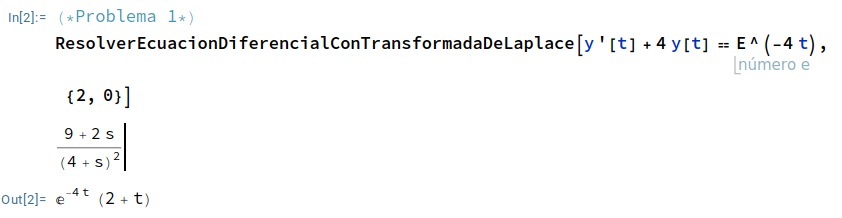
\includegraphics[width=1\textwidth]{../../ED 2/image.png}
\end{center}
\newpage

\subsubsection{Problema 2}
\[y' - y = 1 - te^{t}, \hspace{.5cm} y(0) = 0\]
Aplicamos la Transformada de Laplace a ambos lados de la ecuación:
\[\mathcal{L}\{y'\} - \mathcal{L}\{y\} = \mathcal{L}\{1 - te^{t}\}\]

Utilizamos las siguientes propiedades de la Transformada de Laplace:
\[
    \mathcal{L}\{1\} = \frac{1}{s}, \quad \mathcal{L}\{te^{\alpha t}\} = \frac{1}{(s - \alpha)^2}
\]

Por lo tanto, para \(\mathcal{L}\{1 - te^{t}\}\) tenemos:
\[
    \mathcal{L}\{1\} - \mathcal{L}\{te^{t}\} = \frac{1}{s} - \frac{1}{(s-1)^2}
\]

Para \(\mathcal{L}\{y'\}\) y \(\mathcal{L}\{y\}\), considerando la condición inicial \(y(0) = 0\), obtenemos:
\[
    \mathcal{L}\{y'\} = sY(s) - y(0) = sY(s)
\]
\[
    \mathcal{L}\{y\} = Y(s)
\]

Sustituyendo en la ecuación transformada:
\[
    sY(s) - Y(s) = \frac{1}{s} - \frac{1}{(s-1)^2}
\]

Resolviendo para \(Y(s)\):
\[
    Y(s)(s - 1) = \frac{1}{s} - \frac{1}{(s-1)^2}
\]

\[
    Y(s) = \frac{1}{s(s - 1)} - \frac{1}{(s-1)^3}
\]

Ahora debemos buscar las fracciones parciales de:
\[
    \frac{1}{s(s - 1)} - \frac{1}{(s-1)^3}
\]

Calculamos las fracciones parciales de $\frac{1}{s(s - 1)}$

\[ \frac{1}{s(s - 1)} = \frac{A}{s} + \frac{B}{s-1}\]

\[ 1 = A(s-1) + Bs\]

Para $s=0$

\[ 1 = A(0-1) + B(0)\]

\[ 1 = -A\]

\[A = -1\]

Para $s=1$

\[ 1 = A(1-1) + B(1)\]

\[ 1 = A(0) + B\]

\[ 1 = B\]

\[ \frac{1}{s(s - 1)} = -\frac{1}{s} + \frac{1}{s-1}\]

Ahora aplicamos la tranfsormada inversa de laplace

\begin{align*}
    -\mathcal{L}^{-1}\{\frac{1}{s}\} +  \mathcal{L}^{-1}\{\frac{1}{s-1}\} - \mathcal{L}^{-1}\{\frac{1}{(s-1)^3}\}
\end{align*}

Sabemos:

\[ \mathcal{L}^{-1}[\frac{a}{s}] = a \hspace{1cm} \mathcal{L}^{-1}[\frac{1}{(s-a)^n}] = \frac{t^{n-1}e^{at}}{(n-1)!} \hspace{1cm} \mathcal{L}^{-1}[\frac{1}{s-a}] = e^{at}\]

\begin{align*}
    -\mathcal{L}^{-1}\{\frac{1}{s}\}       & = -1                  \\
    \mathcal{L}^{-1}\{\frac{1}{s-1}\}      & = e^t                 \\
    -\mathcal{L}^{-1}\{\frac{1}{(s-1)^3}\} & = -\frac{t^2e^{t}}{2} \\
\end{align*}

\[-1 + e^t - \frac{t^2e^t}{2}\]

Podemos confirmar este resultado con Mathematica

\begin{center}
    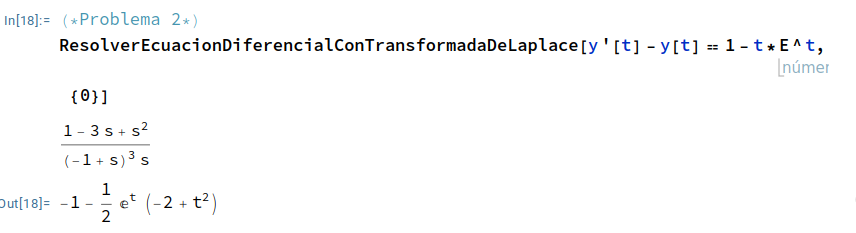
\includegraphics[width=1\textwidth]{../../ED 2/image2.png}
\end{center}

\newpage


\subsubsection{Problema 3}
\[y'' + 2y' + y = 0, \hspace{.5cm} y(0) = y'(0) = 1\]

Aplicamos la Transformada de Laplace a ambos lados de la ecuación:
\[\mathcal{L}\{y''\} + 2\mathcal{L}\{y'\} + \mathcal{L}\{y\} = \mathcal{L}\{0\}\]

Para \(\mathcal{L}\{y''\}\), \(\mathcal{L}\{y'\}\) y \(\mathcal{L}\{y\}\):

\begin{align*}
    \mathcal{L}\{y''\} & = s^2Y(s) - sy(0) - y'(0) \\
    \mathcal{L}\{y'\}  & = sY(s) - y(0)            \\
    \mathcal{L}\{y\}   & = Y(s)
\end{align*}

Considerando la condición inicial \(y(0) = y'(0) = 1\), tenemos:

\begin{align*}
    \mathcal{L}\{y''\} & = s^2Y(s) - s(1) - 1 \\
    \mathcal{L}\{y'\}  & = sY(s) - 1          \\
    \mathcal{L}\{y''\} & = Y(s)
\end{align*}

Sustituyendo:

\[
    s^2Y(s) - s - 1 + 2(sY(s) - 1) + Y(s) = 0
\]

\[
    s^2Y(s) - s - 1 + 2sY(s) - 2 + Y(s) = 0
\]

\[
    Y(s)(s^2 + 2s + 1) - s - 3 = 0
\]

\[
    (s^2 + 2s + 1)Y(s) = s + 3
\]

Despejando $Y(s)$

\[
    Y(s) = \frac{s + 3}{(s + 1)^2}
\]

Calculamos las fracciones parciales

\[
    \frac{s + 3}{(s + 1)^2} = \frac{A}{(s + 1)} + \frac{B}{(s + 1)^2}
\]

\[s+3 = A(s+1) + B\]

Para $s=-1$

\[-1+3 = A(0) + B\]
\[2 = B\]

Para $s-3$

\[-3+3 = A(-3+1) + B\]

\[0 = A(-2) + B\]

Sabemos que $B=2$
\[0 = A(-2) + 2\]
\[-2A = -2\]
\[A = 1\]

\[
    Y(s) = \frac{s + 3}{(s + 1)^2} = \frac{1}{s+1} + \frac{2}{(s+1)^2}
\]

Aplicamos la tranformada inversa de laplace

\begin{align*}
    \mathcal{L}^{-1}\{\frac{1}{s+1}\} +  2\mathcal{L}^{-1}\{\frac{1}{(s+1)^2}\}
\end{align*}

Sabemos:

\[ \mathcal{L}^{-1}[\frac{1}{(s-a)^n}] = \frac{t^{n-1}e^{at}}{(n-1)!} \hspace{1cm} \mathcal{L}^{-1}[\frac{1}{s-a}] = e^{at}\]

\begin{align*}
    \mathcal{L}^{-1}\{\frac{1}{s+1}\}      & = e^{-t}   \\
    2\mathcal{L}^{-1}\{\frac{1}{(s+1)^2}\} & = 2te^{-t} \\
\end{align*}

La solucion es:

\[e^{-t} + 2te^{-t} = e^{-t}(1+2t)\]

Podemos confirmar este resultado con Mathematica

\begin{center}
    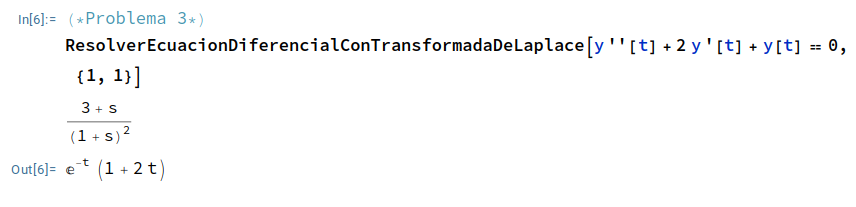
\includegraphics[width=1\textwidth]{../../ED 2/image3.png}
\end{center}

\newpage

\subsubsection{Problema 4}
\[
    y'' - 4y' + 4y = t^{3}e^{2t}, \hspace{.5cm} y(0) = y'(0) = 0
\]

Aplicamos la Transformada de Laplace a ambos lados de la ecuación:
\[
    \mathcal{L}\{y''\} - 4\mathcal{L}\{y'\} + 4\mathcal{L}\{y\} = \mathcal{L}\{t^3e^{2t}\}.
\]

para \(\mathcal{L}\{t^3e^{2t}\}\) tenemos:

\begin{equation*}
    \mathcal{L}\{t^3e^{2t}\} = \frac{3!}{(s-2)^4} = \frac{6}{(s-2)^4}.
\end{equation*}

Para \(\mathcal{L}\{y''\}\), \(\mathcal{L}\{y'\}\) y \(\mathcal{L}\{y\}\):
\begin{align*}
    \mathcal{L}\{y''\} & = s^2Y(s) - sy(0) - y'(0) \\
    \mathcal{L}\{y'\}  & = sY(s) - y(0)            \\
    \mathcal{L}\{y\}   & = Y(s)
\end{align*}

Considerando la condición inicial \(y(0) = y'(0) = 0\), tenemos:
\begin{align*}
    \mathcal{L}\{y''\} & = s^2Y(s) - s(0) - 0 \\
    \mathcal{L}\{y'\}  & = sY(s) - 0          \\
    \mathcal{L}\{y\}   & = Y(s)
\end{align*}

Sustituyendo:
\begin{equation*}
    s^2Y(s) - 4sY(s) + 4Y(s) = \frac{6}{(s-2)^4}.
\end{equation*}

Factorizamos el término en \(Y(s)\) y simplificamos:
\begin{equation*}
    Y(s)(s^2 - 4s + 4) = \frac{6}{(s-2)^4},
\end{equation*}
\begin{equation*}
    Y(s)(s - 2)^2 = \frac{6}{(s-2)^4}.
\end{equation*}

Despejamos \(Y(s)\):
\begin{equation*}
    Y(s) = \frac{6}{(s-2)^6}.
\end{equation*}

Aplicamos la transformada inversa de Laplace:
\begin{align*}
    \mathcal{L}^{-1}\left[\frac{1}{(s-a)^n}\right]  & = \frac{t^{n-1}e^{at}}{(n-1)!} \\
    6\mathcal{L}^{-1}\left[\frac{1}{(s-2)^6}\right] & = 6\frac{t^{5}e^{2t}}{5!}      \\
                                                    & = 6\frac{t^{5}e^{2t}}{120}     \\
                                                    & = \frac{t^{5}e^{2t}}{20}
\end{align*}

Podemos confirmar este resultado con Mathematica

\begin{center}
    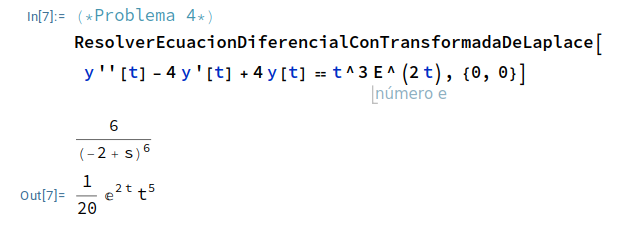
\includegraphics[width=1\textwidth]{../../ED 2/image4.png}
\end{center}


\newpage


\subsubsection{Problema 5}

\[y'' - 6y' + 9y = t, \hspace{.5cm} y(0) = 0, y'(0) = 1\]

Aplicamos la Transformada de Laplace a ambos lados de la ecuación:
\[
    \mathcal{L}\{y''\} - 6\mathcal{L}\{y'\} + 9\mathcal{L}\{y\} = \mathcal{L}\{t\}.
\]

para \(\mathcal{L}\{t\}\) tenemos:

\[\mathcal{L}\{t\}=\frac{1}{s^2}\]

Para \(\mathcal{L}\{y''\}\), \(\mathcal{L}\{y'\}\) y \(\mathcal{L}\{y\}\):
\begin{align*}
    \mathcal{L}\{y''\} & = s^2Y(s) - sy(0) - y'(0) \\
    \mathcal{L}\{y'\}  & = sY(s) - y(0)            \\
    \mathcal{L}\{y\}   & = Y(s)
\end{align*}

Considerando la condición inicial $y(0) = 0$ y $y'(0) = 1$, tenemos:
\begin{align*}
    \mathcal{L}\{y''\} & = s^2Y(s) - s(0) - 1 \\
    \mathcal{L}\{y'\}  & = sY(s) - 0          \\
    \mathcal{L}\{y\}   & = Y(s)
\end{align*}

Sustituyendo:

\[
    s^2Y(s) - 1 - 6sY(s) + 9Y(s) = \frac{1}{s^2}
\]

\[
    Y(s)(s^2 -6s + 9) - 1 = \frac{1}{s^2}
\]

\[
    Y(s)(s^2 -6s + 9) = \frac{1}{s^2} + 1
\]

\[
    Y(s)(s-3)^2 = \frac{1}{s^2} + 1
\]

\[
    Y(s)(s-3)^2 = \frac{1+s^2}{s^2}
\]

\[
    Y(s) = \frac{1+s^2}{s^2(s-3)^2}
\]

Calculamos las fracciones parciales

\[\frac{1+s^2}{s^2(s-3)^2} = \frac{A}{s} + \frac{B}{s^2} + \frac{C}{(s-3)} + \frac{D}{(s-3)^2}\]

\[1+s^2 = As(s-3)^2 + B(s-3)^2 + Cs^2(s-3) + Ds^2\]

Expandiendo:

\[1+s^2 = As^3-6As^2+9As+Bs^2-6Bs+9B+Cs^3-3Cs^2+Ds^2\]
\[1+s^2 = (A+C)s^3+(-6A+B-3C+D)s^2 + (9A-6B)s +9B\]

\begin{align*}
    A+C        & = 0 \\
    -6A+B-3C+D & = 1 \\
    9A-6B      & = 0 \\
    9B         & =1
\end{align*}

DE este sistema observamos:

\[B=\frac{1}{9}\]

Sustituyendo arriba

\[9A - 6(\frac{1}{9}) = 0\]
\[9A = \frac{6}{9}\]
\[A = \frac{6}{81}\]
\[A = \frac{2}{27}\]

Sustituyendo en la primera expresion

\[A + C = 0\]
\[\frac{2}{27} + C = 0\]
\[ C = -\frac{2}{27}\]

Resolviendo la ultima expresion

\[-6A+B-3C+D = 1\]
\[-6(\frac{2}{27})+\frac{1}{9}-3(-\frac{2}{27})+D = 1\]
\[-\frac{12}{27} + \frac{1}{9} + \frac{6}{27} + D = 1\]
\[-\frac{12}{27} + \frac{1}{9} + \frac{6}{27} + D = 1\]
\[-\frac{1}{9} + D = 1\]
\[ D = 1 + \frac{1}{9} = \frac{10}{9}\]

\[\frac{1+s^2}{s^2(s-3)^2} = \frac{2/27}{s} + \frac{1/9}{s^2} + \frac{-2/27}{(s-3)} + \frac{10/9}{(s-3)^2}\]

Aplicar la tranformada inversa de laplace

Sabemos:

\[ \mathcal{L}^{-1}[\frac{a}{s}] = a \hspace{1cm} \mathcal{L}^{-1}[\frac{1}{(s-a)^n}] = \frac{t^{n-1}e^{at}}{(n-1)!} \hspace{1cm} \mathcal{L}^{-1}[\frac{1}{s-a}] = e^{at} \hspace{1cm} \mathcal{L}^{-1}\left[\frac{1}{s^n}\right] = \frac{t^{n-1}}{(n-1)!}
\]

\[\mathcal{L}^{-1}[\frac{2/27}{s}] + \mathcal{L}^{-1}[\frac{1/9}{s^2}] + \mathcal{L}^{-1}[\frac{-2/27}{(s-3)}] + \mathcal{L}^{-1}[\frac{10/9}{(s-3)^2}]\]

\begin{align*}
    \mathcal{L}^{-1}[\frac{2/27}{s}]        & = \frac{2}{27}                                            \\
    \mathcal{L}^{-1}[\frac{1/9}{s^2}]       & = \frac{1}{9} \cdot \frac{t^{2-1}}{(2-1)!} = \frac{1}{9}t \\
    -2/27\mathcal{L}^{-1}[\frac{1}{(s-3)}]  & = \frac{-2}{27}e^{3t}                                     \\
    10/9\mathcal{L}^{-1}[\frac{1}{(s-3)^2}] & = \frac{10}{9}\frac{te^{3t}}{1}
\end{align*}

La tranformada inversa de laplace completa es:

\[\frac{2}{27} + \frac{1}{9}t - \frac{2}{27}e^{3t} + \frac{10}{9}te^{3t}
\]
\newpage


\subsubsection{Problema 6}

\[y'' - 4y' + 4y = t^3, \hspace{.5cm} y(0) = 1, y'(0) = 0\]

Aplicamos la Transformada de Laplace a ambos lados de la ecuación:
\[
    \mathcal{L}\{y''\} - 4\mathcal{L}\{y'\} + 4\mathcal{L}\{y\} = \mathcal{L}\{t^3\}.
\]

para \(\mathcal{L}\{t^3\}\) tenemos:

\[\mathcal{L}\{t^3\} = \frac{6}{s^4}\]

Para \(\mathcal{L}\{y''\}\), \(\mathcal{L}\{y'\}\) y \(\mathcal{L}\{y\}\):
\begin{align*}
    \mathcal{L}\{y''\} & = s^2Y(s) - sy(0) - y'(0) \\
    \mathcal{L}\{y'\}  & = sY(s) - y(0)            \\
    \mathcal{L}\{y\}   & = Y(s)
\end{align*}

Considerando la condición inicial $y(0) = 1$ y $y'(0) = 0$, tenemos:
\begin{align*}
    \mathcal{L}\{y''\} & = s^2Y(s) - s(1) - 0 \\
    \mathcal{L}\{y'\}  & = sY(s) - 1          \\
    \mathcal{L}\{y\}   & = Y(s)
\end{align*}

Sustituyendo:

\begin{align*}
    s^2Y(s) - s - 4(sY(s) - 1) + 4Y(s) & = \frac{6}{s^4}                 \\
    s^2Y(s) - s - 4sY(s) + 4 + 4Y(s)   & = \frac{6}{s^4}                 \\
    s^2Y(s) - 4sY(s) + 4 + 4Y(s)       & = \frac{6}{s^4} + s             \\
    Y(s)(s^2 - 4s + 4) + 4             & = \frac{6}{s^4} + s             \\
    Y(s)(s-2)^2                        & = \frac{6}{s^4} + s - 4         \\
    Y(s)(s-2)^2                        & = \frac{s^5-4s^4+6}{s^4}        \\
    Y(s)                               & = \frac{s^5-4s^4+6}{s^4(s-2)^2}
\end{align*}


Buscamos las fracciones parciales de esta expresion

\[\frac{s^5-4s^4+6}{s^4(s-2)^2} = \frac{A}{s} + \frac{B}{s^2} + \frac{C}{s^3} + \frac{D}{s^4} + \frac{E}{s-2} + \frac{F}{(s-2)^2}\]

podemos calcular las fracciones parciales con \texttt{Mathematica}

\begin{center}
    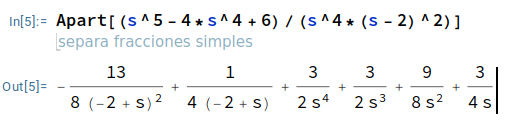
\includegraphics[width=0.6\textwidth]{../../ED 2/image5.png}
\end{center}

\[
    \frac{13}{8 (s-2)^2} + \frac{1}{4 (s-2)} + \frac{3}{2 s^4} + \frac{3}{2 s^3} + \frac{9}{8 s^2} + \frac{3}{4 s}
\]

Calculamos la inversa
\[\mathcal{L}^{-1}[\frac{13}{8 (s-2)^2}] + \mathcal{L}^{-1}[\frac{1}{4 (s-2)}] + \mathcal{L}^{-1}[\frac{3}{2 s^4}] + \mathcal{L}^{-1}[\frac{3}{2 s^3}] + + \mathcal{L}^{-1}[\frac{9}{8 s^2}] + \mathcal{L}^{-1}[\frac{3}{4 s}]\]

\[
    \mathcal{L}^{-1}\left[\frac{13}{8 (s-2)^2}\right] = \mathcal{L}^{-1}\left[\frac{13}{8}\cdot\frac{1}{(s-2)^2}\right] = \frac{13}{8}e^{2t}t \\
\]

\[    \mathcal{L}^{-1}\left[\frac{1}{4 (s-2)}\right] = \mathcal{L}^{-1}\left[\frac{1}{4}\cdot\frac{1}{s-2}\right] = \frac{1}{4}e^{2t} \\
\]

\[\mathcal{L}^{-1}\left[\frac{3}{2 s^4}\right] = \mathcal{L}^{-1}\left[\frac{3}{2}\cdot\frac{1}{s^4}\right] = \frac{3}{2}\cdot\frac{t^3}{3!} = \frac{t^3}{4} \\
\]

\[
    \mathcal{L}^{-1}\left[\frac{3}{2 s^3}\right] = \mathcal{L}^{-1}\left[\frac{3}{2}\cdot\frac{1}{s^3}\right] = \frac{3}{2}\cdot\frac{t^2}{2!} = \frac{3t^2}{4} \\
\]

\[
    \mathcal{L}^{-1}\left[\frac{9}{8 s^2}\right] = \mathcal{L}^{-1}\left[\frac{9}{8}\cdot\frac{1}{s^2}\right] = \frac{9}{8}\cdot\frac{t}{1!} = \frac{9t}{8} \\
\]

\[
    \mathcal{L}^{-1}\left[\frac{3}{4 s}\right] = \mathcal{L}^{-1}\left[\frac{3}{4}\cdot\frac{1}{s}\right] = \frac{3}{4}
\]

\begin{align*}
    y(t) & = \mathcal{L}^{-1}\left[\frac{13}{8 (s-2)^2}\right] + \mathcal{L}^{-1}\left[\frac{1}{4 (s-2)}\right] + \mathcal{L}^{-1}\left[\frac{3}{2 s^4}\right] + \mathcal{L}^{-1}\left[\frac{3}{2 s^3}\right] + \mathcal{L}^{-1}\left[\frac{9}{8 s^2}\right] + \mathcal{L}^{-1}\left[\frac{3}{4 s}\right] \\
         & = \frac{13}{8}e^{2t}t + \frac{1}{4}e^{2t} + \frac{t^3}{4} + \frac{3t^2}{4} + \frac{9t}{8} + \frac{3}{4}
\end{align*}

\begin{center}
    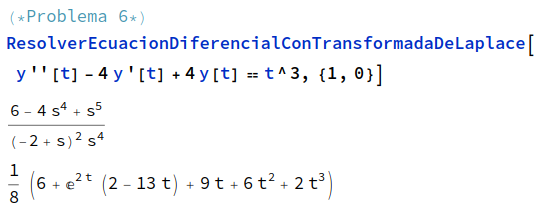
\includegraphics[width=1\textwidth]{../../ED 2/image7.png}
\end{center}


\newpage


\subsubsection{Problema 7}

\[y'' - 6y' + 13y = 0, \hspace{.5cm} y(0) = 0, y'(0) = -3\]

Aplicamos la Transformada de Laplace a ambos lados de la ecuación:
\[
    \mathcal{L}\{y''\} - 6\mathcal{L}\{y'\} + 13\mathcal{L}\{y\} = \mathcal{L}\{0\}
\]

Para \(\mathcal{L}\{y''\}\), \(\mathcal{L}\{y'\}\) y \(\mathcal{L}\{y\}\):
\begin{align*}
    \mathcal{L}\{y''\} & = s^2Y(s) - sy(0) - y'(0) \\
    \mathcal{L}\{y'\}  & = sY(s) - y(0)            \\
    \mathcal{L}\{y\}   & = Y(s)
\end{align*}

Considerando la condición inicial $y(0) = 0$ y $y'(0) = 3$, tenemos:
\begin{align*}
    \mathcal{L}\{y''\} & = s^2Y(s) - s(0) + 3 \\
    \mathcal{L}\{y'\}  & = sY(s) - 0          \\
    \mathcal{L}\{y\}   & = Y(s)
\end{align*}

Sustituyendo:

\[
    s^2Y(s) + 3 - 6sY(s) + 13Y(s) = 0
\]

\[
    Y(s)(s^2 - 6s + 13) + 3 = 0
\]

\[
    Y(s) = -\frac{3}{(s^2 - 6s + 13)} =  -\frac{3}{(s-3)^2+4}
\]

\[
    \quad L\left\{e^{at} \sin(bt)\right\} = \frac{b}{(s - a)^2 + b^2}
\]

\[
    L^{-1}\left\{-\frac{3}{(s-3)^2 + 2^2}\right\} = -3e^{3t} \sin(2t)
\]

\begin{center}
    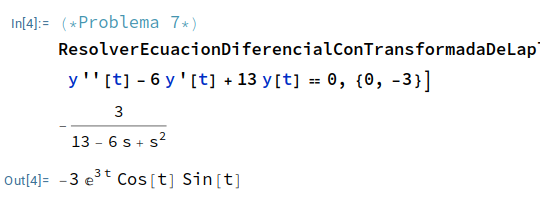
\includegraphics[width=1\textwidth]{../../ED 2/image8.png}
\end{center}

\newpage

\subsubsection{Problema 8}
\[2y'' + 20y' + 51y = 0, \hspace{.5cm} y(0) = 2, y'(0) = 0\]

Aplicamos la Transformada de Laplace a ambos lados de la ecuación:
\[
    2\mathcal{L}\{y''\} + 20\mathcal{L}\{y'\} + 51\mathcal{L}\{y\} = \mathcal{L}\{0\}.
\]

Para \(\mathcal{L}\{y''\}\), \(\mathcal{L}\{y'\}\) y \(\mathcal{L}\{y\}\):
\begin{align*}
    \mathcal{L}\{y''\} & = s^2Y(s) - sy(0) - y'(0) \\
    \mathcal{L}\{y'\}  & = sY(s) - y(0)            \\
    \mathcal{L}\{y\}   & = Y(s)
\end{align*}

Considerando la condición inicial $y(0) = 2$ y $y'(0) = 0$, tenemos:
\begin{align*}
    \mathcal{L}\{y''\} & = s^2Y(s) - s(2) - 0 \\
    \mathcal{L}\{y'\}  & = sY(s) - 2          \\
    \mathcal{L}\{y\}   & = Y(s)
\end{align*}

Sustituyendo:
\[
    2(s^2Y(s) - 2s) + 20(sY(s) - 2) + 51Y(s) = 0
\]

\[
    2s^2Y(s) - 4s + 20sY(s) - 40 + 51Y(s) = 0
\]

\[
    Y(s)(2s^2 + 20s + 51) - 4s - 40 = 0
\]

\[
    Y(s)(2s^2 + 20s + 51) = 4s + 40
\]

\[
    Y(s) = \frac{4s + 40}{2s^2 + 20s + 51}
\]

\[
    Y(s) = \frac{4s + 40}{(s-5)^2+50}
\]

\[
    L^{-1}\left\{\frac{s-a}{(s-a)^2 + \omega^2}\right\} = e^{at} \cos(\omega t)
\]
\[
    L^{-1}\left\{\frac{\omega}{(s-a)^2 + \omega^2}\right\} = e^{at} \sin(\omega t)
\]

\[
    2\left(3\sqrt{2}\sin(5\sqrt{2}t) + 2\cos(5\sqrt{2}t)\right)e^{5t}u(t)
\]


\newpage


\subsubsection{Problema 9}

\[y'' - y' = e^{t}cos(t), \hspace{.5cm} y(0) = 0, y'(0) = 0 \]

Aplicamos la Transformada de Laplace a ambos lados de la ecuación:
\[
    \mathcal{L}\{y''\} - \mathcal{L}\{y'\} = \mathcal{L}\{e^t\cos(t)\}.
\]

Resolviendo $\mathcal{L}\{e^t\cos(t)\}$:

Sabemos:

\[
    \mathcal{L}\{e^{at}\cos(bt)\} = \frac{s-a}{(s-a)^2 + b^2}
\]

\[
    \mathcal{L}\{e^t\cos(t)\} = \frac{s-1}{(s-1)^2 + 1^2}
\]

Para \(\mathcal{L}\{y''\}\), \(\mathcal{L}\{y'\}\) y \(\mathcal{L}\{y\}\):
\begin{align*}
    \mathcal{L}\{y''\} & = s^2Y(s) - sy(0) - y'(0) \\
    \mathcal{L}\{y'\}  & = sY(s) - y(0)
\end{align*}

Considerando la condición inicial $y(0) = 0$ y $y'(0) = 0$, tenemos:
\begin{align*}
    \mathcal{L}\{y''\} & = s^2Y(s) \\
    \mathcal{L}\{y'\}  & = sY(s)
\end{align*}

Sustituyendo:
\[
    s^2Y(s) - sY(s) = \frac{s-1}{(s-1)^2 + 1^2}
\]

\[
    Y(s)(s^2 - s) = \frac{s-1}{(s-1)^2 + 1}
\]

\[
    Y(s) = \frac{s-1}{(s^2 - s)((s-1)^2 + 1)}
\]

\[
    Y(s) = \frac{s-1}{s(s - 1)((s-1)^2 + 1)}
\]

\[
    Y(s) = \frac{1}{s((s-1)^2 + 1)}
\]

\[
    Y(s) = \frac{1}{s^3 - 2s^2 + 2s}
\]

\[
    Y(s) = \frac{1}{s(s^2-2s+2)}
\]

\newpage


\subsubsection{Problema 10}
\[y'' - 2y' + 5y = 1 + t, \hspace{.5cm} y(0) = 0, y'(0) = 4\]

Aplicamos la Transformada de Laplace a ambos lados de la ecuación:
\[
    \mathcal{L}\{y''\} - 2\mathcal{L}\{y'\} + 5\mathcal{L}\{y\} = \mathcal{L}\{1 + t\}
\]

\[
    \mathcal{L}\{y''\} - 2\mathcal{L}\{y'\} + 5\mathcal{L}\{y\} = \frac{1}{s} + \frac{1}{s^2}
\]

Para \(\mathcal{L}\{y''\}\), \(\mathcal{L}\{y'\}\) y \(\mathcal{L}\{y\}\):
\begin{align*}
    \mathcal{L}\{y''\} & = s^2Y(s) - sy(0) - y'(0) \\
    \mathcal{L}\{y'\}  & = sY(s) - y(0)            \\
    \mathcal{L}\{y\}   & = Y(s)
\end{align*}

Considerando la condición inicial $y(0) = 0$ y $y'(0) = 4$, tenemos:

\begin{align*}
    \mathcal{L}\{y''\} & = s^2Y(s) - s(0) - 4 \\
    \mathcal{L}\{y'\}  & = sY(s) - (0)        \\
    \mathcal{L}\{y\}   & = Y(s)
\end{align*}

Sustituyendo:
\[
    s^2Y(s) - 4 - 2sY(s) + 5Y(s) = \frac{1}{s} + \frac{1}{s^2}
\]

\[
    Y(s)(s^2 - 2s + 5) - 4 = \frac{1}{s} + \frac{1}{s^2}
\]

\[
    Y(s)(s^2 - 2s + 5) = \frac{1}{s} + \frac{1}{s^2} + 4
\]

\[
    Y(s)(s^2 - 2s + 5) = \frac{4s^2+s+1}{s^2}
\]

\[
    Y(s) = \frac{4s^2+s+1}{s^2(s^2 - 2s + 5)}
\]

\end{document}